% \documentclass[5p,authoryear,fleqn]{elsarticle}
\documentclass[3p,authoryear,fleqn]{elsarticle}
\journal{ArXiv archiving for pre-publication review}

% *** MISC UTILITY PACKAGES ***
\usepackage[mode=buildnew]{standalone}
\usepackage{gincltex}
\usepackage{glossaries}
\usepackage{booktabs} % to use \toprule
\usepackage{multirow}
\usepackage[colorinlistoftodos]{todonotes}
\usepackage{xifthen}
\usepackage{xspace}
\usepackage{graphicx}
\graphicspath{{figures/}}

%\usepackage[cmex10,intlimits]{amsmath}
\usepackage{amsmath}
\usepackage{amssymb}
%\usepackage{algorithmic}
\DeclareMathOperator{\tr}{tr}
\DeclareMathOperator{\argmax}{argmax}
\DeclareMathOperator{\argmin}{argmin}
\DeclareMathOperator{\diag}{diag}
\DeclareMathOperator{\dist}{dist}
\DeclareMathOperator{\const}{Const.}
\providecommand{\e}[1]{\ensuremath{\times 10^{#1}}}
\providecommand{\mdist}[2]{ \mathcal{D}_{#2}^2(\mathbf{#1}) }
\providecommand{\omegaset}{\ensuremath{\boldsymbol{\Omega}}}
\providecommand{\gammaset}{\ensuremath{\boldsymbol{\Gamma}}}
\providecommand{\regseg}{\emph{regseg}}
\providecommand{\Regseg}{\emph{Regseg}}

\let\oldhat\hat
\renewcommand{\vec}[1]{\mathbf{#1}}

\providecommand{\nvec}[1]{\hat{\mathbf{#1}}}
\providecommand{\suppl}[1]{\href{http://dx.doi.org/mydoi}{Supplemental Materials}, #1}
\providecommand{\isores}[2][]{#2\ensuremath{\times}#2\ensuremath{\times}#2%
\ifthenelse{\equal{#1}{}}{}{ [#1]}\xspace}

% *** PDF, URL AND HYPERLINK PACKAGES ***
%
\usepackage{url}
\usepackage[colorlinks=true,linkcolor=black, citecolor=blue, urlcolor=blue]{hyperref}
\usepackage{doi}

% correct bad hyphenation here
\hyphenation{op-tical net-works semi-conduc-tor an-isot-ropy regis-tra-tion iso-tropic Free-Surfer %
align-ed pre-sent work-flow data-set data-sets}

% List of acronyms used in the text
\newacronym{mr}{MR}{magnetic resonance}
\newacronym{mri}{MRI}{magnetic resonance imaging}
\newacronym{dwi}{dMRI}{diffusion MRI}
\newacronym{dw}{DW}{diffusion weighted}
\newacronym{dti}{DTI}{diffusion tensor imaging}
\newacronym{t1}{T1}{T1-weighted}
\newacronym{t2}{T2}{T2-weighted}
\newacronym{csf}{CSF}{cerebrospinal fluid}
\newacronym{wm}{WM}{white matter}
\newacronym{gm}{GM}{grey matter}
\newacronym{epi}{EPI}{echo-planar imaging}
\newacronym{gre}{GRE}{gradient echo sequence}
\newacronym{fa}{FA}{fractional anisotropy}
\newacronym{md}{MD}{mean diffusivity}
\newacronym{acwe}{ACWE}{active contours without edges}
\newacronym{map}{MAP}{maximum a posteriori}
\newacronym{snr}{SNR}{signal-to-noise ratio}
\newacronym{pve}{PVE}{partial volume effect}
\newacronym{roi}{ROI}{region of interest}
\newacronym{mrf}{MRF}{Markov Random Field}

\newacronym{se}{SE}{Surface error}
\newacronym{wi}{WI}{Warping index}
\newacronym{nof}{NoF}{number of fibers}



\makeglossaries

%\acrodef{mr}[MR]{magnetic resonance}
%\acrodef{mri}[MRI]{magnetic resonance imaging}
%\acrodef{dwi}[DWI]{diffusion weighted imaging}
%\acrodef{dw}[DW]{diffusion weighted}
%\acrodef{dti}[DTI]{diffusion tensor imaging}
%\acrodef{t1}[T1]{T1-weighted}
%\acrodef{t2}[T2]{T2-weighted}
%\acrodef{csf}[CSF]{cerebrospinal fluid}
%\acrodef{wm}[WM]{white matter}
%\acrodef{gm}[GM]{grey matter}
%\acrodef{epi}[EPI]{echo-planar imaging}
%\acrodef{fa}[FA]{fractional anisotropy}
%\acrodef{md}[MD]{mean diffusivity}
%\acrodef{acwe}[ACWE]{active contours without edges}
%\acrodef{map}[MAP]{maximum a posteriori}
%\acrodef{snr}[SNR]{signal-to-noise ratio}
%\acrodef{pve}[PVE]{partial volume effect}
%\acrodef{roi}[ROI]{region of interest}


\usepackage[T1]{fontenc}
\usepackage{charter}
%\usepackage[expert]{mathdesign}
%\usepackage[libertine,cmintegrals,cmbraces,vvarbb]{newtxmath}
%\renewcommand*{\familydefault}{\sfdefault}

\usepackage{array}
\newcolumntype{L}[1]{>{\raggedright\let\newline\\\arraybackslash\hspace{0pt}}m{#1}}

\usepackage{ifpdf}

\ifpdf
  \usepackage[switch]{lineno}
  % nothing to do
\else
  \makeatletter
  \def\temp{dvips.def}
  \ifx\Gin@driver\temp
  \def\Ginclude@graphics#1{\def\temp{#1}---image \expandafter\strip@prefix\meaning\temp---}
  \fi
  \makeatother
\fi


% http://tex.stackexchange.com/questions/56105/missing-references-heading
\def\bibsection{\section*{References}}
\begin{document}
\begin{frontmatter}

%% Use \dochead if there is an article header, e.g. \dochead{Short communication}
% \dochead{Preprint for ArXiv archiving and pre-submission review}

\title{Active contours-driven registration method for the structure-informed segmentation of diffusion MR images}

\author[bit,ciber]{Oscar~Esteban\corref{corrauthor}}
\cortext[corrauthor]{Corresponding author}
\ead{phd@oscaresteban.es}
\author[ucla]{Dominique~Zosso}
\author[scil,lts5]{Alessandro~Daducci}
\author[chuv,lts5]{Meritxell~Bach-Cuadra}
\author[bit,ciber]{Mar\'ia-J.~Ledesma-Carbayo}
\author[lts5]{Jean-Philippe~Thiran}
\author[bit,ciber]{Andres~Santos}


\address[bit]{Biomedical Image Technologies (BIT), ETSI Telecomunicaci\'on, Universidad Polit\'ecnica de Madrid, Madrid, Spain}
\address[ciber]{Centro de Investigaci\'on Biom\'edica en Red en Bioingenier\'ia, Biomateriales y Nanomedicina (CIBER-BBN), Zaragoza, Spain}
\address[ucla]{Department of Mathematics, University of California,
Los Angeles (UCLA), Los Angeles, CA, US}
\address[scil]{Computer Science Department, Faculty of Science, Universit\'e de Sherbrooke, 2500 Boulevard Universit\'e, Sherbrooke, QC J1K 2R1, Canada}
\address[lts5]{Signal Processing Laboratory (LTS5), \'Ecole Polytechnique
F\'ed\'erale de Lausanne (EPFL), Lausanne, Switzerland}
\address[chuv]{Dept. of Radiology, CIBM, University
Hospital Center (CHUV) and University of Lausanne (UNIL), Lausanne, Switzerland}

\begin{abstract}
% -*- root: 00-main.tex -*-
\newcomment[RV\#1(C.1)\par RV\#2(C.10)]{%
Current methods using diffusion MRI to map the microstructure and connectivity of the
  human brain increasingly require precise delineations of anatomical structures.
The problem is typically solved by projecting the structural information extracted
  in T1-weighted images, by means of nonlinear registration since diffusion
  MRI data present geometrical distortions.
Here we propose \regseg{}, which segments homogeneous regions within multivariate
  images by projecting a set of nested surfaces extracted from structural images.}
The surfaces evolve through a free-form deformation field supported by the B-spline basis
  to optimally map the contours onto the data in the target space.
We tested the functionality of \regseg{} using four digital phantoms warped with known and
  randomly generated deformations, where subvoxel accuracy was achieved.
\newcomment[RV\#2(C.11)]{%
We proposed a set of surfaces that define a segmentation model of the fractional anisotropy and
  the apparent diffusion coefficient maps derived from diffusion MRI datasets.}
These surfaces extracted from the same-subject T1-weighted image successfully segmented 16 real
  diffusion MRI datasets from the Human Connectome Project that were warped by realistic and nonlinear
  distortions.
We computed the misregistration error of the surfaces estimated by \regseg{} with respect
  to their theoretical location using the ground truth, thereby obtaining a 95\% CI of 0.56--0.66 mm
  distance between corresponding mesh vertices, which was below the 1.25 mm isotropic resolution of the images.
We also compared the performance of the proposed method with a widely used registration tool, which showed
  that \regseg{} outperformed this method in our settings.
\end{abstract}

% Note that keywords are not normally used for peerreview papers.
\begin{keyword}
active~contours \sep cortical~parcellation \sep diffusion MRI \sep nonlinear~registration \sep segmentation \sep susceptibility~distortion.
\end{keyword}

\end{frontmatter}

\linenumbers
% -*- root: 00-main.tex -*-
\section{Introduction}
\label{sec:introduction}

Nonlinear registration of images is a challenging task ubiquitous
  in an endless number of image analysis applications.
The process aims to find a spatial mapping $U$ that aligns the information available
  in two different coordinate systems (generally called
  \emph{reference}, $R$, and \emph{moving}, $M$):
  \begin{align}
  U\colon R \subset \mathbb{R}^n &\to M \subset \mathbb{R}^n \notag\\
  \vec{r} &\mapsto \vec{r}' =\vec{r}+u(\vec{r}),
  \label{eq:transform}
  \end{align}
  where $\vec{r}$ denotes a position in the reference domain $R$, $\vec{r}'$ is
  its corresponding location in $M$, and $n$ the dimensionality of images.
Finally, $\vec{u} = u(\vec{r})$ is the displacement of every point with respect
  to the reference domain.
A comprehensive survey by \citeauthor{sotiras_deformable_2013} \citep{sotiras_deformable_2013}
  illustrates the wide variety of existing registration methodologies.
They classify the algorithms by the three principal building blocks that can be identified
  among methods: the matching criteria or similarity function to evaluate the proximity of
  the solution, the deformation model that may implement theoretical properties and constraints
  of the mapping in the selected application, and the optimization method or search strategy.
The most widespread matching criteria are probably the so-called \emph{iconic
  methods} \citep{sotiras_deformable_2013}.
These algorithms require the definition of an appropriate function on the voxel-wise information
  content of both images.
A second group, called \emph{geometric methods}, measure distances between features derived from
  corresponding objects defined in both spaces, such as landmarks, shapes, surfaces, etc.
Finally, \emph{hybrid methods} combine properties of the iconic and geometric methods.
As reviewed in \citep{sotiras_deformable_2013}, an important research effort has been devoted to
  study application-oriented matching criteria.


Currently uprising applications, such as the extraction of connectivity networks from
  diffusion \gls*{mri} \citep{craddock_imaging_2013}, demand for improved approaches
  that outperform existing techniques.
We propose the image registration -based solution to correct for the
  susceptibility distortions in \gls*{dmri} of the brain ,
  that is involved in the extraction of the structural connectivity map of the brain.
However they are not appropriate for all the registration problems
  \citep{greve_accurate_2009}.
They propose a \emph{hybrid method} \citep{sotiras_deformable_2013} for the
  intra-subject registration of \gls*{t1} \gls*{mri} and \gls*{dmri} images
  of the brain using a linear transformation model.
As in \citep{greve_accurate_2009}, we exploit the precise structures that
  can be readily extracted with widely-used tools at high resolution
  and map this prior information to low resolution data,
  in which the scale of the imaged structures is in the range of the image
  resolution or above.
Our approach differs with \citep{greve_accurate_2009} in two fundamental
  choices: 1) We use a nonlinear deformation model that enables the
  correction of the susceptibility-derived distortions
  \citep{jezzard_correction_1995} that \gls*{dmri} data typically present.
And 2) our matching criteria does not necessarily need for clear intensity
  steps at the tissue interfaces where surfaces must be fitted.

The hypothesis underpinning this research is that, in those situations,
  image registration can be reliably performed by searching for homogeneous
  regions in one image corresponding to a prior knowledge of the shape of objects in
  the moving coordinate system.


%{\color{red} {The main diverging points with respect to
%\citep{gorthi_active_2011} are: 1) there is no need for an explicit level set function
%$\Phi_G$, as we replace the level set gradient computation $N_{\Phi_G}$ with shape
%gradients \citep{besson_dream2s_2003,herbulot_segmentation_2006};
%2) regularization is also based on linear diffusion smoothing \citep{thirion_image_1998},
%but we replace the Gaussian filtering by other constraints
%studied in \citep{nagel_investigation_1986} to better the problem;
%3) optimization is applied in the spectral
%domain, observing anisotropic and inhomogeneous mappings along each direction.
%With respect \citep{guyader_combined_2011}, the main differences are
%the distance function, and the spectral solution to the optimization updates,
%as we shall cover in \autoref{sec:numerical_implementation}.}}



%In this paper we formulate the joint registration-segmentation
%problem as follows.
%such that the known contours in anatomical space $T$ optimally segment
%the diffusion space $D$.
%
%
%Whereas related \glspl*{adf} introduced in \autoref{sec:methods_background}
%make use of explicit level-set formulations to solve \eqref{eq:gradient_descent},
%we alternatively use \emph{shape-gradients}
%\cite{besson_dream2s_2003,herbulot_segmentation_2006}.

%
%Let us denote by $\vec{x}$ the voxel and $F(\vec{x}) = [ f_1, f_2, \ldots, f_N]^T$
%  its associated feature vector in the following.
%
%In our application, these surfaces are precise tissue interfaces of interest extracted
%  from a high-resolution, anatomically correct reference volume using
%  the well-established
%
%In this paper we propose a novel registration framework to simultaneously
%solving the segmentation, distortion and cortical parcellation challenges,
%by exploiting as strong shape-prior the detailed morphology extracted
%from high-resolution and anatomically correct \gls{mri}.
%Indeed, hereafter
%we assume this segmentation problem in anatomical images is reliably and
%accurately solved with readily available tools (e.g.
%\citep{fischl_freesurfer_2012}).
%After global alignment with \gls{t1} using existing approaches, the remaining
%spatial mismatch between anatomical and diffusion space is due to susceptibility
%distortions.
%Finally, we need to establish precise spatial correspondence between the
%surfaces in both spaces, including the tangential direction for parcellation.
%Therefore, we can reduce the problem to finding the differences of spatial
%distortion in between anatomical and \gls{dwi} space.
%We thus reformulate the segmentation problem as an inverse problem, where we
%seek for an underlying deformation field (the distortion) mapping
%from the structural space into the diffusion space, such that the structural
%contours segment optimally the \gls{dwi} data.
%In the process, the one-to-one
%correspondence between the contours in both spaces is guaranteed, and projection
%of parcellisation to \gls{dwi} space is implicit and consistent.
%
%We test our proposed joint segmentation-registration model on two different
%synthetic examples.
%The first example is a scalar sulcus model, where the
%\gls{csf}-\gls{gm} boundary particularly suffers from \gls{pve} and can only be
%segmented correctly thanks to the shape prior and its coupling with the inner,
%\gls{gm}-\gls{wm} boundary through the imposed deformation field regularity.
%The second case deals with more realistic \gls{dwi} data stemming from
%phantom simulations of a simplistic brain data.
%Again, we show that the
%proposed model successfully segments the \gls{dwi} data based on two derived
%scalar features, namely \gls{fa} and \gls{md}, while establishing an estimate
%of the dense distortion field.
%
%The rest of this paper is organized as follows.
%First, in \autoref{sec:methods}
%we introduce our proposed model for joint multivariate segmentation-registration.
%Then we provide a more detailed description of the data and experimental setup in
%\autoref{sec:experiments}.
%We present results in \autoref{sec:results} and conclude
%in \autoref{sec:conclusion}.
%
%
%The properties of the reconstructed tensors and derived scalar maps have
%been studied by \cite{ennis_orthogonal_2006}. Based on their
%findings, \gls{fa}~\eqref{eq:fa} and \gls{md}~\eqref{eq:md} are
%considered complementary features, and therefore we selected them for the
%energy model \eqref{eq:complete_energy} in driving the
%registration-segmentation process.
%Whereas \gls{fa} informs mainly about the \emph{shape} of diffusion,
%the \gls{md} is more related to the \emph{magnitude} of the process:
%
%\begin{align}
%\mathrm{FA} &= \sqrt{ \frac{1}{2}}\,\frac{\sqrt{ (\lambda_1 - \lambda_2)^2 + (\lambda_2 - \lambda_3)^2 + (\lambda_3 - \lambda_1)^2}}{\sqrt{ {\lambda_1}^2 + {\lambda_2}^2 + {\lambda_3}^2}} \label{eq:fa} \\
%\mathrm{MD} &= ( \lambda_1 + \lambda_2 + \lambda_3 ) / 3 \label{eq:md}
%\end{align}
%where $\lambda_i$ are the eigenvalues of the diffusion tensor
%associated with the diffusion signal $S(\vec{q})$. There exist
%two main reasons to justify their choice.
%First, they are well-understood and standardized in clinical routine.
%Second, together they contain most of the information that is
%usually extracted from the \gls{dwi}-derived scalar maps
%\cite{ennis_orthogonal_2006}.
%

% -*- root: 00-main.tex -*-
\section{Methods}
\label{sec:methods}
%

\subsection{Susceptibility-derived distortions}
\label{sec:distortions}
\Gls*{dmri} data are usually acquired with \gls*{epi} schemes.
In order to quickly probe the diffusion process within the brain in many different orientations,
  these sequences minimize the bandwidth of the \gls*{pe} direction.
This low bandwidth originates the artifactual displacement of locations presenting small deviations
  from the main magnetic field $B_0$.
One important source of these deviations ($\Delta B_0$) is the discontinuity of magnetic
  susceptibility across the imaged object.
Tissue/air boundaries show large steps of susceptibility and this artifact is
  particularly evident in the surroundings of the orbito-frontal lobe or the temporal
  bone of both hemispheres.
Distortion can be rendered as a registration problem between the undistorted $R$ (reference), 
  and distorted $M$ (moving) spaces:

  \begin{align}
  U_s\colon R \subset \mathbb{R}^n &\to M \subset \mathbb{R}^n \notag\\
  \vec{r} &\mapsto \vec{r}' =\vec{r}+u(\vec{r}),
  \label{eq:transform}
  \end{align}
%
  where $\vec{r}$ denotes a position in $R$, $\vec{r}'$ is
  its corresponding location in $M$, and $n$ the dimensionality of images.
Finally, $\vec{u} = u(\vec{r})$ is the displacement of every point with respect
  to the reference domain.

The displacements field $U_s$ along the \gls*{pe} axis can be estimated theoretically
  \citep{jezzard_correction_1995}:

  \begin{equation}
  \vec{r}' = \vec{r} + \frac{\gamma \, T_{acq}\, s_{PE}}{2\pi}\Delta B_0(\vec{r}) \cdot \hat{\vec{e}}_{PE},
  \label{eq:fieldmap}
  \end{equation}
%
where $\gamma$ is the gyromagnetic ratio, $T_{acq}$ is the readout time,
  $s_{PE}$ is the pixel size along \gls*{pe}, and $\hat{\vec{e}}_{PE}$ the unitary
  vector along \gls*{pe}.
Several methodologies have been proposed to estimate $U_s$ and fix the artifact.
The first solution consisted on estimating $\Delta B_0$ with field mapping
  techniques \citep{andersson_modeling_2001}.
A second family of methods require an extra \gls*{epi} acquisition, but switching
  the \gls*{pe} axis \citep{chiou_simple_2000} or reversing the direction of gradient \gls*{pe}
  increments \citep{cordes_geometric_2000,holland_efficient_2010}.
\cite{kybic_unwarping_2000} proposed nonlinear registration of the \emph{b0}
  image\footnote{The term \emph{b0} refers to one or more images within the
  \gls*{dmri} dataset that are acquired with a null or very low gradient intensity or
   \emph{b}-value.} of the \gls*{dmri} to an undistorted \gls*{t2} image of
   the same subject.
In the following, we will refer to this method as \gls*{t2b}.
Further developments \citep{irfanoglu_susceptibility_2011} extended the \gls*{t2b} 
  approach to the 3D problem.
Therefore, a typical protocol for the extraction of structural connectivity
  comprehends \gls*{dmri}, \gls*{t1}, and the acquisition determined by the correction
  method of choice \citep{daducci_connectome_2012}.


\subsection{Our method and contributions}
\label{sec:contributions}
%
\emph{Regseg} can be viewed as a derivation of \emph{bbregister} \citep{greve_accurate_2009}.
Both methods exploit the anatomically correct and precise surfaces that are readily
  extracted with \emph{FreeSurfer} \citep{fischl_freesurfer_2012}, mapping them
  to a target \gls*{dmri} image using active contours.
We implemented active contours without edges \citep{chan_active_2001}, that allow
  \emph{regseg} to segment homogeneous regions within the brain, while \emph{bbregister}
  use active contours with edges to look for intensity boundaries in the target image.
Another identifying difference is the deformation model:
  \emph{bbregister} includes an affine transformation and overcomes the distortion
  problem by excluding typically affected regions from computation.
Conversely, \emph{regseg} implements a free-deformation field supported with B-Spline
  functions.
Our method is close to \citep{guyader_combined_2011} and \citep{gorthi_active_2011}
  in the use of active contours without edges for registration, however we avoided
  the use of level sets with the application of shape gradients
  \citep{besson_dream2s_2003,herbulot_segmentation_2006}.
\cite{gorthi_active_2011} used a gaussian regularizer, and \cite{guyader_combined_2011}
  proposed a nonlinear elasticity smoother.
In contrast, \emph{regseg} implements the anisotropic regularization proposed by
  \citep{nagel_investigation_1986}.
We also present an ellaborated evaluation instrumentation to create realistic distortions
  and test algorithms.
Integrating \emph{regseg} and an in-house implementation of the \gls*{t2b} correction
  in the workflow, we compared the performance of both solutions.


\subsection{Cost-function derivation}\label{sec:methods_map}
%
In a Bayesian framework, the mappings $U$ in \eqref{eq:transform} are
  evaluated based on their posterior probability given the observed data
  $R$.
Using the Bayes' rule, the posterior likelihood is computed as:

  \begin{equation}
  P(U \mid R,\Gamma_{l,m}) = \frac{P(R \mid U,\Gamma_{l,m})\, P(U)}{P(R)},
  \label{eq:bayes_rule}
  \end{equation}
%
  where $P(R \mid U,\Gamma_{l,m})$ is the data-likelihood, and
  $\Gamma_{l,m}$ are a set of surfaces corresponding to the interfaces
  between piecewise smooth regions $\Omega_i$, such that
  $\Gamma_{l,m} = \partial \Omega_l \cap \partial \Omega_m$ is the
  contour between competing regions $\Omega_l$ and $\Omega_m$.
The best estimate $\hat{U}$ then fulfills the maximum a posteriori criterium
  \citep{bishop_pattern_2006}, and aligns $\Gamma$ into $R$.

First, we assume independence between pixels, and thus break down the
  global data likelihood into a product of pixel-wise conditional probabilities:

  \begin{equation}
  P(R \mid U,\Omega) = \underset{l}{\prod} \underset{\vec{r}\in \Omega_l}{\prod}
    P\left( \vec{f}' \mid U \right),
  \label{eq:bayes_aposteriori}
  \end{equation}
%
  where $\vec{f}' = R(\vec{r}')$ is the feature vector at the displaced
  position $\vec{r}'$ \eqref{eq:transform} in the multispectral target
  volume.
For convenience, and because it has been shown to be an appropriate approximation
  \citep{leemput_automated_1999,cuadra_comparison_2005}, we introduce two assumptions for each
  region $\Omega_l$:
  1) the features are i.i.d.; and 2) they can be modeled by multivariate normal
  distributions with parameters $\lbrace \boldsymbol{\mu}_l, \boldsymbol{\Sigma}_{l} \rbrace$
  for each region $\Omega_l$.
We then insert the normal distribution into \eqref{eq:bayes_rule} to obtain the full
  formulation of the \emph{data term} of our registration model:

 	\begin{align}
  P( R \mid U, \Omega ) &= \underset{l}{\prod} \underset{\vec{r} \in \Omega_l}{\prod}
  \mathcal{N} ( \vec{f} \mid \boldsymbol{\mu}_l, \boldsymbol{\Sigma}_{l} ) \notag\\
  &= \underset{l}{\prod} \underset{\vec{r} \in \Omega_l}{\prod} \frac{1}{ \sqrt{(2\pi)^{C}\,\left|\boldsymbol{\Sigma}_{l}\right|}}\,{e^{\left(-\frac{1}{2}
  \mdist{f'}{l} \right)}},
  \label{eq:pdf}
  \end{align}
%
  using $\mdist{f}{l}$ to denote the squared \emph{Mahalanobis distance} of $\vec{f}$ with respect
  to the descriptors of region $l$ as
  $\mdist{f}{l} = (\vec{f} - \boldsymbol{\mu}_l)^T \, {\boldsymbol{\Sigma}_l}^{-1} \, (\vec{f} - \boldsymbol{\mu}_l)$.


The smoothness of the resulting displacements field is induced by a Thikonov regularization
  prior:

  \begin{align*}
  P(U) = \underset{\vec{r}}{\prod}\, p(\vec{u}) &=
  \underset{\vec{r}}{\prod}\, p_0(\vec{u}) \, p_1(\vec{u}), \\
  p_0(\vec{u}) &= \mathcal{N}( \vec{u} \mid 0, \mathbf{A}^{-1}), \notag\\
  p_1(\vec{u}) &= \mathcal{N}(  \nabla \vec{u} \mid 0, \mathbf{B}^{-1}),
  \end{align*}
%
  imposing that the distortion and its gradient have zero
  mean and variance governed by the matrices $\mathbf{A} = (a_{ij})$ and $\mathbf{B} = (b_{ij})$.
Since the anisotropy is generally aligned with the imaging axes, $\mathbf{A}$ and $\mathbf{B}$
  can be simplified to diagonal matrices.
For convenience, we will set $\alpha_i = a_{ii}^2$ and $\beta_i = b_{ii}^2$, what can be reduced
  using the Hadamard square root notation\footnote{The Hadamard power of a matrix or a vector
  is the power of its elements $\mathbf{M}^{\circ p} = ({m_{ij}}^{p})$} as
  $\mathbf{A}=\boldsymbol{\alpha}^{\circ\frac12}\,\vec{I}_n$ and
  $\mathbf{B}=\boldsymbol{\beta}^{\circ\frac12}\,\vec{I}_n$.


Finally, the maximum a posteriori problem is adapted into a variational one where we look for
  the minimum of an energy functional, by applying a log-transform:

  \begin{align}
  E(R \mid U) &= -\log \underset{l}{\prod}
  \underset{\vec{r} \in \Omega_l}{\prod}
  \mathcal{N} \left( \vec{f}' \mid \Theta_l \right)\,p_0( \vec{u})\,p_1( \vec{u}) \notag\\
  &= C + \underset{l}{\sum} \int_{\Omega_l}
  \mdist{f'}{l} \,d\vec{r} \notag\\
  &+ \int_{\Omega} \left[ \boldsymbol{\alpha} \cdot \vec{u}^{\circ2}
  + \boldsymbol{\beta} \cdot (\nabla \vec{u})^{\circ2} \right] \,d\vec{r},
  \label{eq:energy}
  \end{align}
%
  this expression is dual to the energy functional corresponding
  to a discrete \gls*{acwe} framework \citep{chan_active_2001}
  with the corresponding anisotropic regularization term \citep{nagel_investigation_1986}.


\subsection{Numerical Implementation}
\label{sec:numerical_implementation}

\begin{figure}
	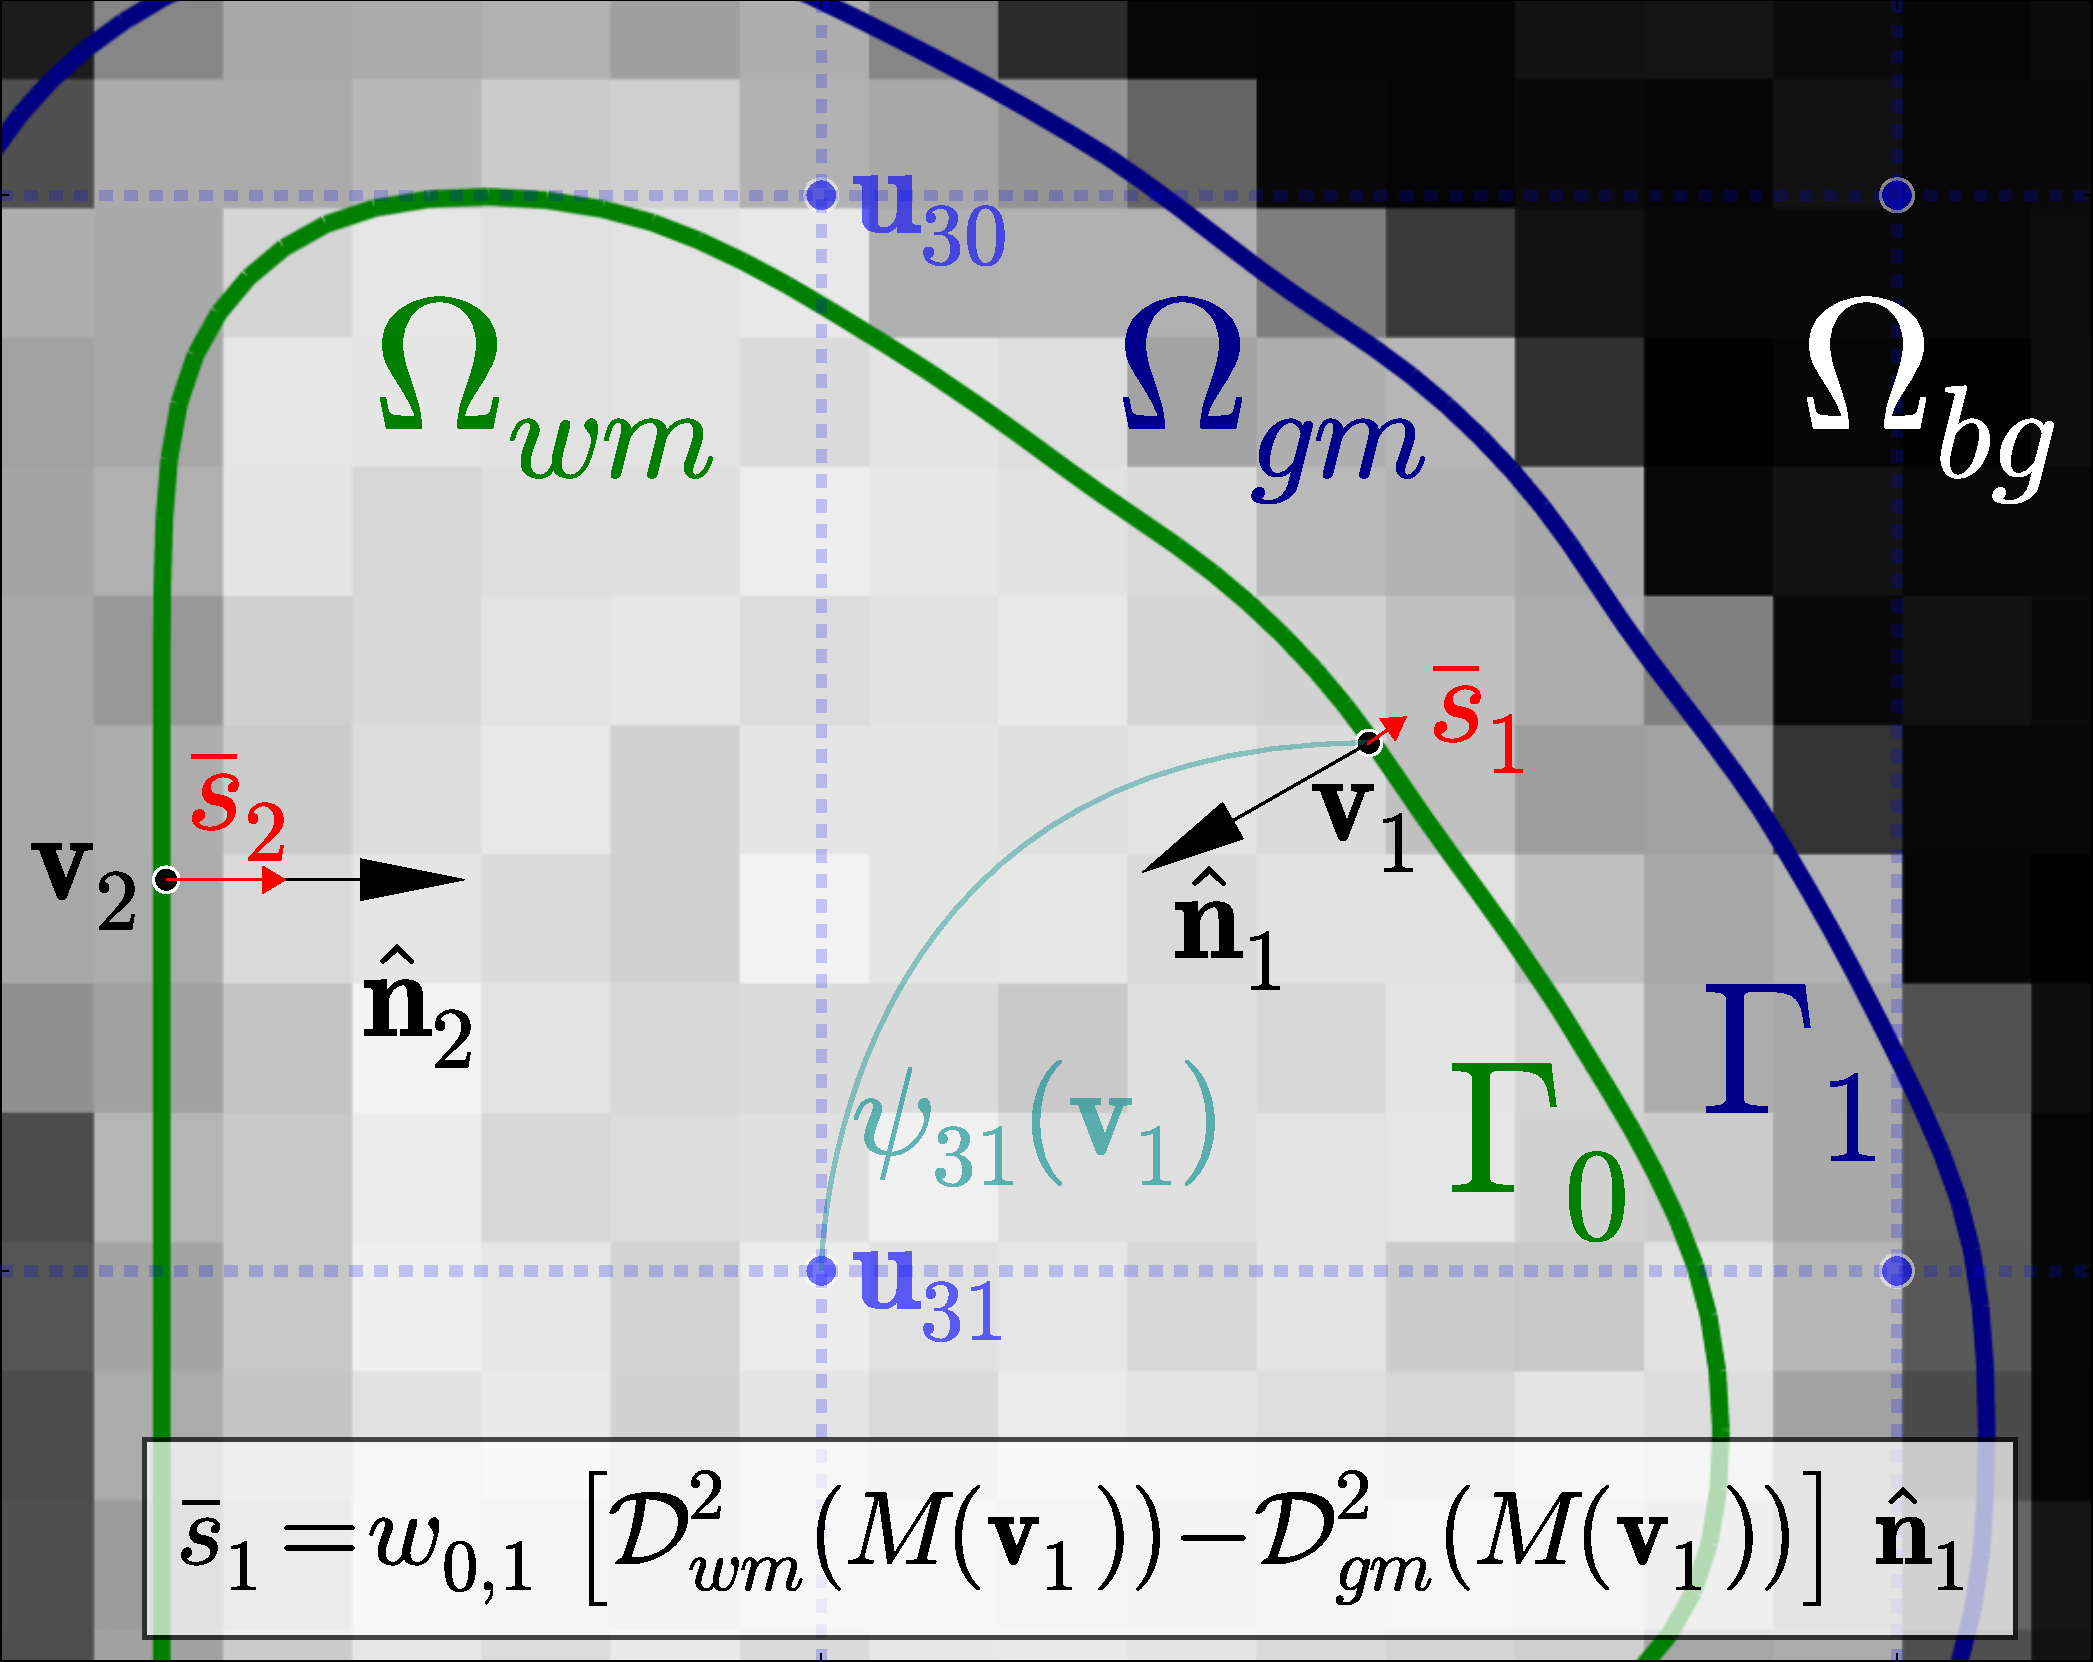
\includegraphics[width=\linewidth]{figures/figure01}
	\caption{The active contours are defined as the interfacing surfaces of the competing
	  \glspl{roi} $\Omega_i$.
	They are represented in green and dark blue colors in this close-up.
	They iteratively evolve following their inner normals $\hat{n}_i$ at each vertex
	  $\vec{v}_i$ of the mesh.
	The gradient speeds $\bar{s}_i$ are computed as the disparity between data energies of
	  the vertex $\vec{v}_i$ in each limiting region (see \ref{app:shape_priors}).
	In this figure, the gradient speed corresponding to $\vec{v}_1$ is written in the lower
	  box, $\Omega_{wm}$ being the inner limiting region and $\Omega_{gm}$ the outer.
	Finally, every $\bar{s}_i$ is associated with the control points $\vec{u}_k$ through
	  the corresponding weights $\psi_k(\vec{v}_i)$ by Eq. \eqref{eq:gradient_wshape}.
	}\label{fig:method}
\end{figure}

\paragraph*{Deformation model}\label{sec:deformation_model}
Let us denote $\{\vec{v}_i\}_{i=1 \ldots N_c}$ the vertices of one or several prior
  surface(s).
In our application, these surfaces are triangularized meshes extracted using \emph{FreeSurfer}
  \citep{fischl_freesurfer_2012}.
The transform $\hat{U}$ \eqref{eq:transform} is supported by a dense deformation field
  $\vec{u} = u(\vec{r})$, such that:

  \begin{equation}
  \vec{v}_i' = \hat{U}\{\vec{v}_i\} = \vec{v}_i + u(\vec{v}_i) = \vec{v}_i + \vec{u}_i.
  \label{eq:nodes_tfm}
  \end{equation}

Since the nodes of the anatomical surfaces likely lay off-grid, it is required to
  derive $u(\vec{r})$ from a discrete set of parameters $\{\vec{u}_k\}_{k=1 \ldots K}$.
Densification is achieved through a set of associated basis functions $\psi_k$:

  \begin{equation}
  u(\vec{r}) = \sum_k \psi_k(\vec{r}) \vec{u}_k.
  \label{eq:intp_kernel}
  \end{equation}

In our implementation, $\psi_k$ is chosen to be a tensor-product B-Spline kernel
  of degree 3 ($\beta_3$).
Then, introducing \eqref{eq:intp_kernel} into \eqref{eq:nodes_tfm} and replacing
  $\psi$ by the actual kernel function, the transformation writes:

  \begin{equation}
    \vec{v}_i' = \vec{v}_i + \sum_k \left[ \vec{u}_k \, \underset{d}{\prod}
      \beta_3( (\vec{v}_i - \vec{r}_k) \cdot \hat{\mathbf{e}}_d ) \right],
  \label{eq:transformation}
  \end{equation}
%
  with $\hat{\mathbf{e}}_d$ being the unitary vector along axis $d$.


\paragraph*{Optimization}
\label{sec:gradient_descent}
To find the minimum of the energy functional \eqref{eq:energy},
  we propose a gradient-descent approach with respect to the underlying
  deformation field through the following \gls*{pde}:

  \begin{equation}
  \frac{\partial u(\vec{r},t)}{\partial t} \propto - \frac{\partial E(R \mid U)}{\partial \vec{u}_k},
  \label{eq:general_gradient_descent}
  \end{equation}
%
  with $t$ being an artificial time parameter of the contour
  evolution, and $\vec{u}_k$ the parameters supporting the estimate
  $\hat{U}$ of the transformation at the current time point.
Now, we introduce \eqref{eq:energy} in \eqref{eq:general_gradient_descent}:

  \begin{align}
  \frac{\partial E(\vec{u})}{\partial \vec{u}_k} &=
  \frac{ \partial }{\partial \vec{u}_k} \Big\{
  \int_{\Omega} \underset{l}{\sum} \mdist{f'}{l} \,d\vec{r} \notag\\
  &+ \int_{\Omega} [ \boldsymbol{\alpha} \cdot \vec{u}^{\circ2}
  + \boldsymbol{\beta} \cdot (\nabla \vec{u})^{\circ2} ] \,d\vec{r}
  \Big\}.
  \label{eq:gradient_descent}
  \end{align}


We apply a discretized interpretation of \eqref{eq:shape_gradients} to compute
  the data term in \eqref{eq:gradient_descent} using shape-gradients
  \citep{herbulot_segmentation_2006}, and ultimately avoid level sets.
We refer the reader to the appendix \autoref{app:shape_priors} in order to fill in the gap
  between \eqref{eq:gradient_descent} and the following expression:

  \begin{align}
  \frac{\partial E_{data}(\vec{u})}{\partial \vec{u}_k} &=
  \frac{ \partial }{\partial \vec{u}_k} \left\{
   \underset{\vec{x} \in \Omega_l}{\sum} \underset{l}{\sum} \mdist{f'}{l} \right\} \notag\\
  &= \underset{i}{\sum} w_i
   \left\langle \frac{\partial \vec{v}_i'}{\partial \vec{u}_k}, \bar{s}_i'\right\rangle,
  \label{eq:gradient_wshape}
  \end{align}
%
  in this case, the formulation has been adapted to the non-binary case, $\{l,m\}$
    being any pair of neighboring regions, and $\Gamma_{l,m}$ the contour separating
    them such that
    $\vec{x}' = \vec{v}' \in\Gamma_{l,m} \iff \vec{x}\in \partial\Omega_i \cap \partial\Omega_j$,
    $\bar{s}_i'$ is the speed vector projected on to the unit inward normal to the contour
    at $c_i'$ (described in \autoref{fig:method}), $w_i$ is the area contribution of vertex
    $c_i'$ to the the total area of the surface it belongs.


Finally, we can compute:

  \begin{align}
  \frac{\partial \vec{v}_i'}{\partial \vec{u}_k} &= \frac{\partial}{\partial \vec{u}_k}
  \left\{ \vec{v}_i + \sum_k \psi_k(\vec{v}_i) \vec{u}_k \right\}
  = \psi_k(\vec{v}_i)\, \hat{\vec{e}}
  \label{eq:basis_derivative}
  \end{align}
%
  where $\hat{\vec{e}}$ is the coordinates system's unit vector.
The vertex speeds $\bar{s}_i'$ obtained by computing the shape-gradients \eqref{eq:shape_gradients},
	are then projected to the deformation field in order to obtain the derivatives $\vec{g}_k$
	corresponding to $\vec{u}_k$:

  \begin{equation}
  \vec{g}_{i,k} = w_i \, \left\langle \frac{\partial}{\partial \vec{u}_k}{\vec{v}_i}', \bar{s}_i'\right\rangle
  = - w_i \left[ \mdist{f_i'}{l} - \mdist{f_i'}{m} \right] \psi_k(\vec{v}_i)\, \hat{\vec{n}}_i,
  \end{equation}
%
  then the full gradient evolution equation \eqref{eq:gradient_descent} yields:

  \begin{align}
  \frac{\partial E(\vec{u}_k)}{\partial \vec{u}_k} =
  &\underset{i}{\sum} \vec{g}_{i,k} +2\, \boldsymbol{\alpha} \vec{u}_k
  -2\, \boldsymbol{\beta} \Delta \vec{u}_k,
  \label{eq:gradient_final}
  \end{align}

Finally, we introduce a step size parameter $\delta$ to discretize the artificial time parameter
  in the iterative optimization.
Then, applying the Fourier transform as detailed in the \suppl{section S1}, the
  update equation is derived from \eqref{eq:gradient_final}:

  \begin{align}
  \vec{u}_k^{t+1} = \mathcal{F}^{-1}\left\{ \frac{\mathcal{F}\{\vec{u}_k^t / \delta - \sum_i \vec{g}_{i,k}\}}%
                  {\mathcal{F}\{(1/\delta+\boldsymbol{\alpha})I-\boldsymbol{\beta}\Delta\}} \right\}
  \label{eq:update_equation}
  \end{align}


\paragraph*{Settings, implementation details, and convergence}
\label{sec:conv_report}
The registration parameters (such as $\delta$, $\boldsymbol{\alpha}$, $\boldsymbol{\beta}$,
  the B-Spline grid resolutions, target image smoothing, etc.)
  and other implementation details (for instance the sparse matrix approach
  to fast interpolation) are discussed in the \suppl{section S1}.
The actual choices of parameter settings are publicly distributed with the source code of the experiments.
Additionally, we release our software along with a tool for generating convergence reports to
  demonstrate the behavior of \emph{regseg} and help scientists configure their own experiments.
One sample report is found in the \suppl{section S1.3}.


\subsection{Experiments and evaluation}
\label{sec:experiments_evaluation}
%
In order to demonstrate the performance of \emph{regseg}, we first conducted a battery of
  accuracy tests over synthetic data, and then applied it in the susceptibility distortion
  correction of real data.
\autoref{fig:evworkflows} presents the workflow implementing the evaluation instruments.
Besides a visual assessment of the results, we report quantitative evaluations using
  two metrics.
In the case of the phantoms, since we had produced distortions along the three
  available dimensions, we computed the Haussdorf distance, by reusing the
  ``point-to-cell'' method of \cite{commandeur_vtk_2011}.
Conversely, the susceptibility-derived distortions only happen along the \gls*{pe}
  axis of the image.
Therefore, a \gls*{swindex} can be computed as the one-to-one distance between corresponding
  vertices of surfaces, weighted by their respective Voronoi area $a_i$:

  \begin{equation}
  sWI = \frac{1}{P} \sum\limits_p^P \frac{1}{A_p} \sum\limits_i^{N_p} a_i\,\|
  \vec{v}_i - \hat{\vec{v}}_i \|
  \label{eq:swindex}
  \end{equation}
%
  where $\vec{v}_i$ are the locations of the $N_p$ vertices in each $p \in \{1, \dots P\}$
  prior, $A_p$ the total area of surface $p$, and $\hat{\vec{v}}_i$ is the location
  recovered corresponding to the vertex $\vec{v}_i$.


\begin{figure*}
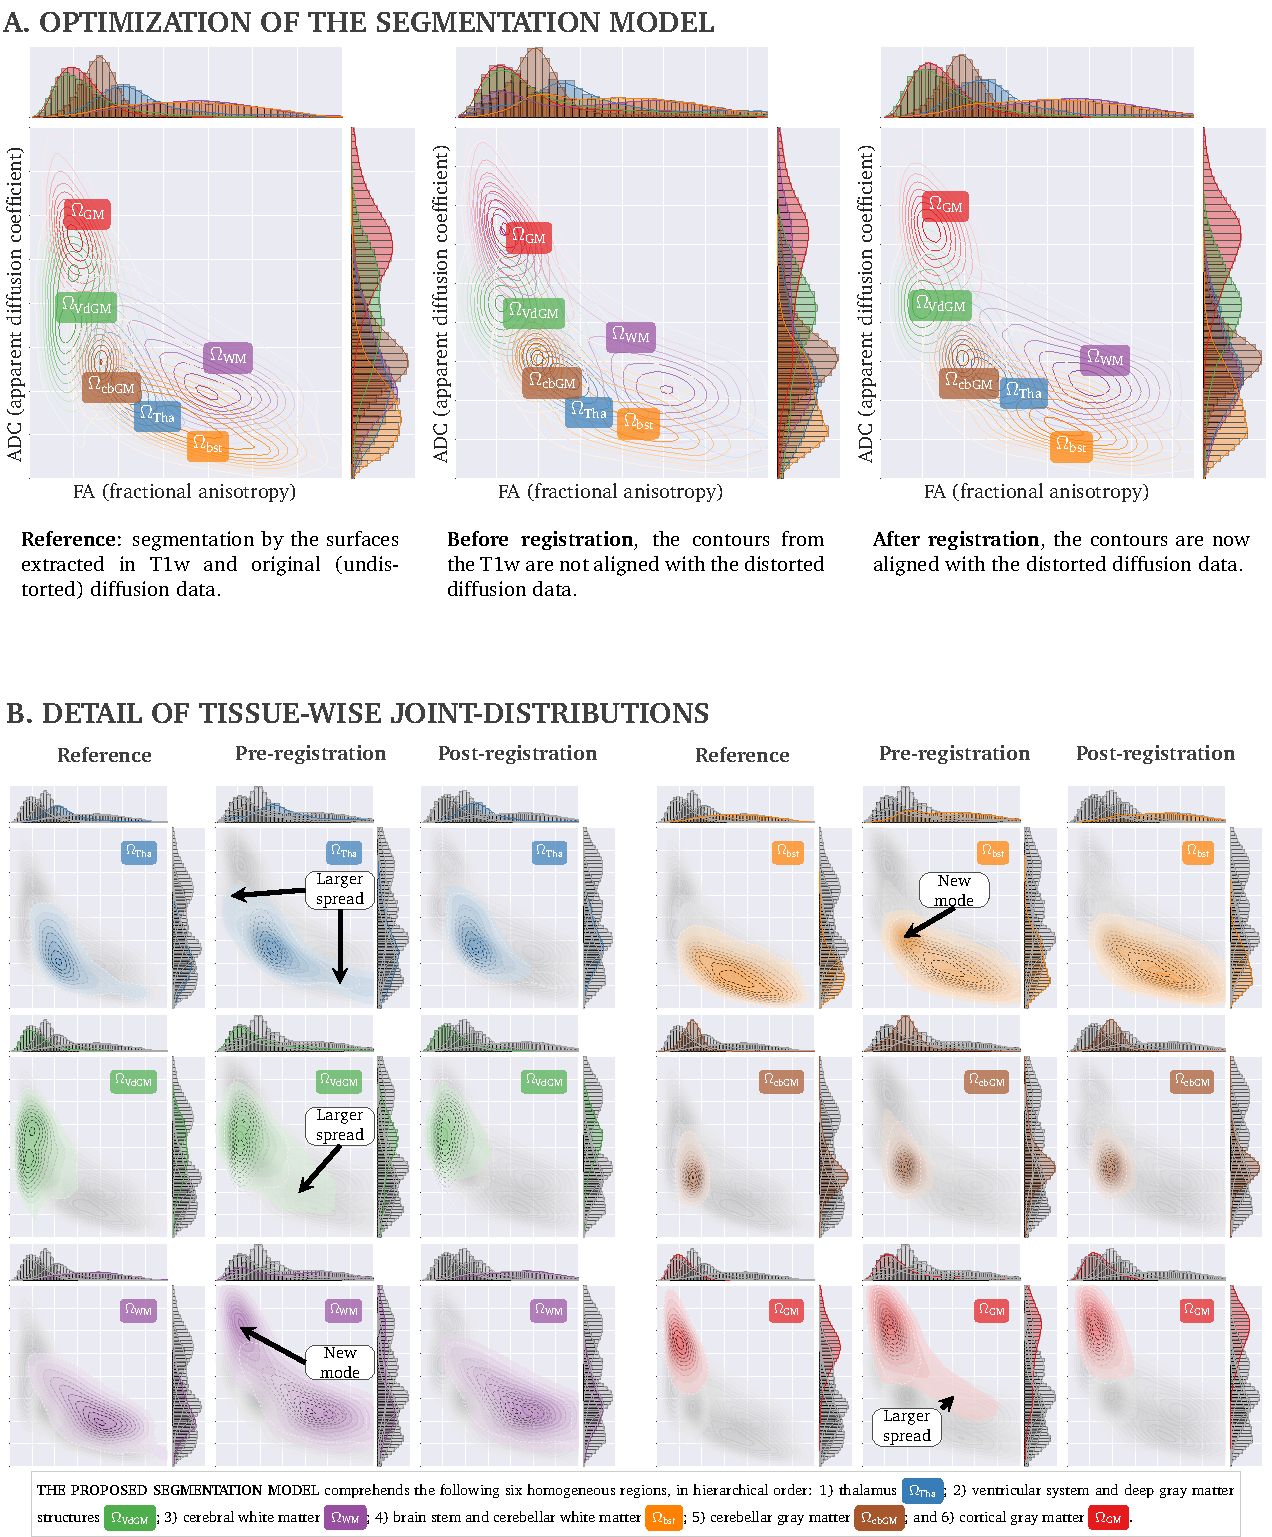
\includegraphics[width=\linewidth]{figures/figure02}
\caption{Experimental workflow applied on real data from the \acrfull*{hcp}.
  1) The prior surfaces are extracted from the anatomical reference (\gls*{t1} image).
	2) To operate as ground truth, we generate a plausible-synthetic distortion $U_{true}$
	  from the fieldmap using \eqref{eq:fieldmap}.
	3) The \gls*{dmri} data are warped using $U^{-1}_{true}$ to reproduce the effects of real
	  susceptibility-derived distortions.
	Target diffusion scalars (\gls*{fa} and \gls*{adc}) are computed on the distorted data and
		stacked to feed the multivariate input required by our algorithm.
	4) \emph{Regseg} is run, obtaining a $U_{test} = \hat{U}_{true}$, the estimation of
	  the ground-truth deformation.
	5) Results are visually and quantitatively evaluated.}\label{fig:evworkflows}
\end{figure*}


\subsection{Image Data and preprocessing}
\label{sec:datasets}

\paragraph*{Simulated phantoms}%
\label{sec:digital_phantoms}
We proved the concept on simplistic digital phantoms which we will name after their
  appearance as ``box'', ``ball'', ``L-shape'', and ``gyrus'' (\autoref{fig:phantom},
  boxes A and B).
Using \emph{phantomas} \citep{caruyer_phantomas_2014}, we simulated
  \gls*{t1} (TE/TR=10/1500ms) and \gls*{t2} images (TE/TR=90/5000ms)
  corresponding to each phantom type, with two resolutions each
  ($1.0mm$ and $2.0mm$ isotropic).
Simulations were corrupted with rician noise for a \gls*{snr} of 300.0.
The reference surfaces were extracted at the higher resolution (1.0mm isotropic),
  using \texttt{mri\_tessellate}\footnote{A marching-cubes algorithm shipped with 
  \emph{FreeSurfer} \citep{fischl_freesurfer_2012}}.

\begin{figure*}
	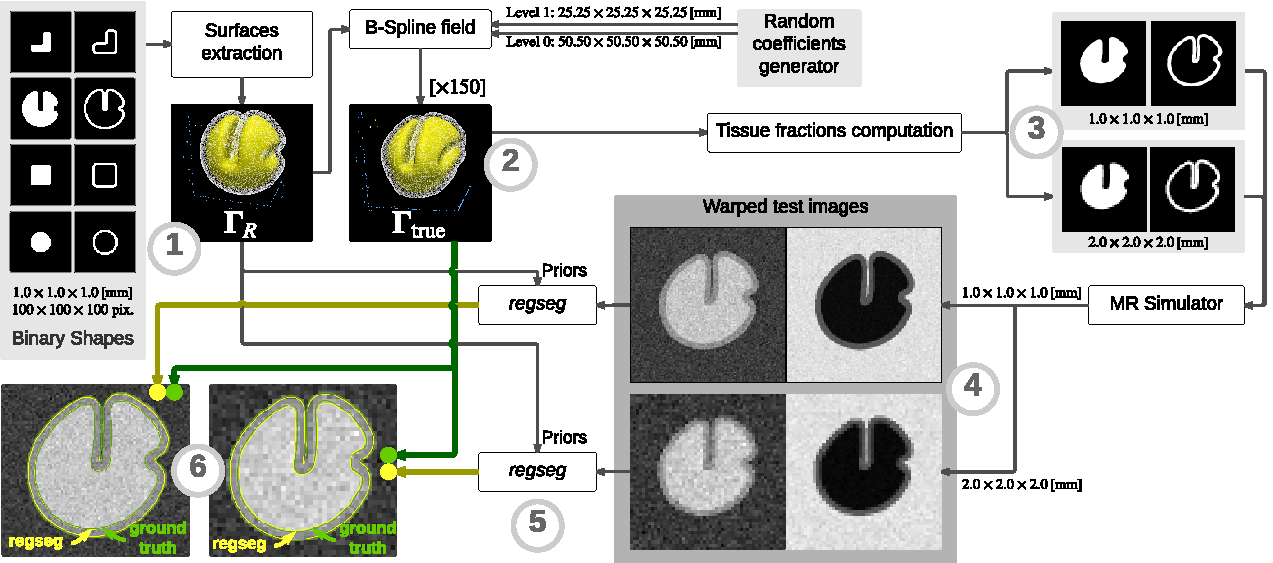
\includegraphics[width=\linewidth]{figures/figure03}
	\caption{A. The ``cortex'' phantom is a spherical shape with two sulci and an
	  outer crust resembling the cortical folding (left).
	The model is used to generate \gls*{t1} and \gls*{t2} images after warping the
	  contours using a random and plausible transformation $U_{true}^{-1}$ (right).
	B. Visual assessment of the results on the low resolution sets:
	  ``gyrus'' (top-left), ``L-shape'' (top-right), ``ball'' (bottom-left),
	  and ``box'' at (bottom-right).
	In yellow color, the recovered contours after registration are represented.
	Our method showed high accuracy, as demonstrates almost exact location of the registered
    contours with respect to their ground truth position depicted in green.
	Partial volume effect turns segmentation of the sulci a challenging problem with voxel-wise
	  clustering methods, but it is successfully segmented with our method.
	C. Quantitative evaluation of registration error in terms of average Hausdorff distance of
	  surfaces at high (left) and low (right) resolutions, demonstrating that the error is
	  consistently below the voxel size.
	  }\label{fig:phantom}
\end{figure*}

To warp the simulated datasets, we generated 150 different realizations of
  the distortion $U_{true}$.
Smoothness is introduced using two levels of B-Spline functions, with control points evenly
  located in isotropic grids covering the full extent of the phantom.
The first level had $50.5mm$ of separation between control points and the second $25.25mm$.
The rationale behind this choice is producing large deformations on the contours with
  the first level, and matching the properties of susceptibility-derived distortions
  as previously reported by \cite{irfanoglu_susceptibility_2011} with the finer grid.
The coefficients of the B-Spline functions were randomly generated for each resolution level.
Invertibility of $U_{true}$ is ensured by controlling the maximum displacement at each
  level ($20.2mm$ and $10.1mm$ respectively) as studied in \citep{rueckert_diffeomorphic_2006}.

\paragraph*{Real datasets} %
\label{sec:human_connectome}
%
For the evaluation of the algorithm on real \gls*{dmri} data of human brains,
  we collected 16 datasets from the ``minimally preprocessed''
	 database of the \gls*{hcp}.
We refer the reader to \citep{essen_human_2012} for exact details about acquisition
  parameters, and \citep{glasser_minimal_2013} for the preprocessing issues.
The datasets comprehend a large set of images, containing \gls*{t1}, \gls*{t2} and
  multi-shell \gls*{dmri} images.
The original acquisitions are released within ``unprocessed'' packages, and
  the ``minimally preprocessed'' are corrected for artifacts, brain-extracted
  and spatially normalized, along with some results of the standard processing
  pipeline of \emph{FreeSurfer}.

Selecting the appropriate labels in the \emph{aparc} segmentation, we applied
  \texttt{mri\_tessellate} to extract the surface of the following
  six homogeneous regions $\Omega_l$:
  1) the thalamus, $\Gamma_{Tha}$;
  2) \gls*{csf} of the ventricular system and deep \gls*{gm} structures, $\Gamma_{VdGM}$;
  3) cerebral \gls*{wm}, $\Gamma_{WM}$;
  4) brain stem and cerebellar \gls*{wm}, $\Gamma_{bst}$;
	5) cerebellar \gls*{gm}, $\Gamma_{cbGM}$; and
	6) cortical \gls*{gm} surface, $\Gamma_{pial}$.
The choice of this particular model is further addressed in \autoref{sec:res_model_and_metric}.

In this case, we derived the deformation $U_{true}$ from the field maps released with
  the corresponding packages of each dataset from the \gls*{hcp} applying \eqref{eq:fieldmap},
  mimicking the real distortions, using a derivation of our previous work
  \citep{esteban_simulationbased_2014}.
After warping the original \gls*{dmri} with $U_{true}^{-1}$, we computed the \gls*{dti} and
  the derived scalars (\gls*{fa} and \gls*{adc}) using \emph{MRtrix} \citep{tournier_mrtrix_2012}.
The stack of \gls*{fa} and \gls*{adc} conforms the multivariate input for \emph{regseg}.

A dual workflow to the general evaluation framework (\autoref{fig:evworkflows})
  was also implemented to integrate the \gls*{t2b} registration scheme.
We reproduced the solution and settings provided with \emph{ExploreDTI}
  \citep{leemans_exploredti_2009}, a widely used toolkit for tractography analysis of
  \gls*{dti}.
\emph{ExploreDTI}, internally uses \emph{elastix} \citep{klein_elastix_2010} to
  perform registration.
First, the average \emph{b0} volume is computed using all the \emph{low-b} volumes within
  the distorted \gls*{dmri} dataset.
Using the ``preprocessed'' instance of the \gls*{t2} image of the corresponding subject as
  reference image, and the \emph{b0} image as moving image, we registered both and
  projected the correct (undistorted) contours to the warped space using the resulting
  transform.
% -*- root: 00-main.tex -*-
\section{Results}
\label{sec:regseg-results}

\subsection{Verification and validation using digital phantoms}
\label{sec:regseg-results_phantom}

The results summarized in \autoref{fig:regseg-phantom} demonstrated that the accuracy was
  high and below the image resolution.
Panel B on \autoref{fig:regseg-phantom} shows the violin plots for each model type corresponding
  to the two sets of resolutions for the generated phantoms.
In order to relate the average misregistration error to the resolution of the moving image,
  we proceeded as follows.
First, we confirmed that the vertex-wise error distributions were skewed by using Shapiro-Wilk's test of
  normality.
All of the distributions of errors in the tests (four phantom types $\times$ two resolutions) were
  non-normal with $p<$ 0.001.
Consequently, we used the non-parametric Wilcoxon signed-rank test with the Bonferroni
  correction for multiple comparisons ($N$=150, for each phantom type).
The average errors were significantly lower than the voxel size with $p <$ (0.001 / 150)
  in all tests (four phantom types $\times$ two resolutions).
Statistical tests might not be sufficiently conclusive, so we also computed the confidence intervals,
  as shown in \autoref{tab:ci_phantom}.

\begin{figure*}[!h]
  \centering
  \includestandalone[width=\linewidth]{figure05}
  \caption{A. Visual assessment of the results obtained with the low resolution sets:
    ``gyrus'' (top left), ``L'' (top right), ``ball'' (bottom left),
    and ``box'' at (bottom right).
  The contours recovered after registration are represented in yellow.
  \Regseg{} achieved high accuracy because it determined the almost exact locations of the registered
    contours with respect to their ground truth positions (shown in green).
  The partial volume effect makes segmentation of the sulci a challenging problem with voxel-wise
    clustering methods, but they were successfully segmented with \regseg{}.
  B. Quantitative evaluation of registration errors in terms of the average Hausdorff distances between
    surfaces at low (left) and high (right) resolutions, which demonstrate that the errors were
    consistently below the size of the voxels.
    }\label{fig:regseg-phantom}
\end{figure*}
\begin{figure*}[!h]
  \centering
  \includestandalone[width=\linewidth]{figure06}
  \caption{A. Example of a visual assessment report, which was automatically generated by the evaluation tool.
    Each view shows one component of the input image (in this case, the \gls*{fa} map), the ground-truth locations
    of the surfaces (green contours), and the resulting surfaces obtained with the test method (yellow contours).
  The first two rows show axial slices for \regseg{} and the \acrfull*{t2b} method, while the last two rows
    show the corresponding sagittal views.
  The coronal view is omitted because it was the least informative due to the directional property
    of the distortions.
  Specific regions where \regseg{} outperformed \gls*{t2b} are enlarged.
  B. Violin plots of the error distributions for each surface, which show the voxel size of the \gls*{dmri} images
    (1.25 mm), thereby supporting the improved results obtained by \regseg{} with the proposed settings.
  }\label{fig:regseg-results_real}
\end{figure*}

\subsection{Evaluation using real datasets and cross-comparison}\label{sec:regseg-results_hcp}
Finally, we compared the performance of \regseg{} with that of the standard \gls*{t2b}
  method.
Summary reports for visual assessment of the 16 cases are included in the
  \citetalias[section S5]{esteban_useful_2015}.
In \autoref{fig:regseg-results_real}, box A, the visual report is shown for one subject.
We computed the \gls*{swindex} \eqref{eq:regseg-swindex} of every surface after registration
  using both the \regseg{} and \gls*{t2b} methods.
Finally, to compare the results, we performed Kruskal-Wallis H-tests
  (a non-parametric alternative to ANOVA) on the warping indices for the three surfaces of
  interest selected in \autoref{sec:regseg-experiments_evaluation}
  ($\Gamma_{VdGM}$, $\Gamma_{WM}$, $\Gamma_{pial}$).
All of the statistical tests showed that the error distributions obtained with \regseg{} and
  \gls*{t2b} were significantly different, and the violin plots in box B of
  \autoref{fig:regseg-results_real} demonstrate that the errors were always larger with \gls*{t2b}.
We also show the 95\% CIs of the \gls*{swindex} for these surfaces.
The aggregate CI for \regseg{} was 0.56--0.66 [mm], whereas the \gls*{t2b} method
  yielded an aggregate CI of 2.05--2.39 [mm].
The results of the statistical tests and the CIs are summarized in \autoref{tab:results_real}.

\begin{table}
\centering
\footnotesize
\tabcolsep=0.1cm
\begin{minipage}{.48\textwidth}
    \vskip-4.7ex
    \begin{tabular}{lccccc}
    Res.   & ``gyrus'' & ``ball''  & ``box''   & ``L''     & Aggreg.    \\\hline
    1.0mm  & 0.18--0.38 & 0.31--0.45 & 0.34--0.42 & 0.34--0.40 & 0.34--0.38  \\
    2.0mm  & 0.59--0.60 & 0.65--0.76 & 0.68--0.71 & 0.67--0.77 & 0.64--0.66  \\
    \hline
    \end{tabular}
    \caption{The distributions of vertex-wise Hausdorff distances between the ground-truth surfaces and their
    corresponding estimates obtained with \regseg{} presented a 95\% CI below the half-voxel size for all of
    the phantom types.
    The CIs were computed by bootstrapping using 10$^\text{4}$ samples, with the median as the location statistic.}\label{tab:ci_phantom}
\end{minipage}
\hfill
\begin{minipage}{.48\textwidth}
    \begin{tabular}{cccccc}
    & & $\Gamma_{VdGM}$  & $\Gamma_{WM}$ & $\Gamma_{pial}$ & Aggreg. \\
    \hline
    \multirow{2}{*}{CI}
       & \regseg{} & 0.50--0.78 & 0.50--0.55 & 0.66--0.73 & 0.56--0.66 \\
       & T2B       & 1.78--2.58 & 1.94--2.36 & 2.16--2.58 & 2.05--2.39 \\
    \hline
    \multirow{2}{*}{H-tests}
       & p-value  & 4.1\e{-6} & 2.3\e{-6} & 2.3\e{-6} & 1.8\e{-16} \\
       & H-stat   & 21.20 & 22.31 & 22.31 & 67.85 \\
    \hline
    \end{tabular}
    \caption{Statistical analysis of results obtained using real data, which show that \regseg{} performed better than
    the alternative \acrfull{t2b} method.
    The distribution of the errors computed for the surfaces of interest ($\Gamma_{VdGM}$, $\Gamma_{WM}$, $\Gamma_{pial}$)
      and the aggregate of all surfaces (Aggreg. column) had lower 95\% CIs with \regseg{}.
   The CIs in this table were computed by bootstrapping using the mean as the location statistic and with 10$^\text{4}$ samples.
    The Kruskal-Wallis H-tests indicated that there was a significant difference between the results obtained using \regseg{} and
      the \gls*{t2b} method.
    }\label{tab:results_real}
\end{minipage}
\end{table}
% -*- root: 00-main.tex -*-
\section{Discussion}
\label{sec:regseg-discussion}
We present \regseg{}, a simultaneous segmentation and registration method that
  maps a set of nested surfaces into a multivariate target-image.
The nonlinear registration process evolves driven by the fitness of the
  picewise-smooth classification of voxels in the target volume imposed
  by the current mapping of the surfaces.
We propose \regseg{} to incorporate anatomical information extracted from \gls*{t1}
  images into the corresponding \gls*{dmri} of the same subject.
Previously, joint segmentation and registration has been applied successfully to
  other problems such as longitudinal object tracking \citep{paragios_level_2003}
  and atlas-based segmentation \citep{gorthi_active_2011}.
The most common approach to solve the problem simultaneously is optimizing a deformation
  model (registration) that supports the evolution the active contours (segmentation),
  like \cite{paragios_level_2003,yezzi_variational_2003}.
\Regseg{} can be seen as a particular case of atlas-based segmentation, replacing the atlas
  by the structural image of the subject (\emph{structure-informed segmentation}).
However, the majority of atlas-based segmentation methods, such as \citep{gorthi_active_2011},
  use a multiphase level set function to register several active contours.
Alternatively, \regseg{} implements the active contours with a hierarchical set of explicit
  surfaces (triangular meshes) that substitute the multiphase level sets, and registration
  is driven by shape-gradients \citep{herbulot_segmentation_2006}.

An important antecedent of \regseg{} is \emph{bbregister} \citep{greve_accurate_2009}.
The tool has been widely adopted as the standard registration method to be used along with the \gls*{epi}
  correction of choice.
It implements a linear mapping, and uses 3D active contours \emph{with edges} to
  search for intensity boundaries in the \lowb{} image.
The active contours are initialized using surfaces extracted from the \gls*{t1} using
  \emph{FreeSurfer} \citep{fischl_freesurfer_2012}: the \emph{pial} surface (exterior of the
  cortical \gls*{gm}) and the \emph{white} surface (the \gls*{wm}/\gls*{gm} interface).
The \lowb{} image only includes a detectable frontier for the pial surface, and thus
  \emph{bbregister} is limited to align the pial contour in this application.
To overcome the problem of nonlinear distortions, \emph{bbregister} excludes the
  regions that are typically warped from the boundary search.
Indeed, the distortion must be addressed separately because it is not supported by
  the affine transformation model.
Conversely, the deformation model of \regseg{} is nonlinear and the active contours are
  \emph{without-edges} \citep{chan_active_2001}.
The contours are without edges because the \gls*{fa} and \gls*{adc} maps do
  not present steep image gradients (edges) but the anatomy can be identified
  by looking for piece-wise smooth homogeneous regions.


Recently, \cite{guyader_combined_2011} proposed a simultaneous segmentation and
  registration method in 2D using level sets and a nonlinear elasticity smoother on the
  displacement vector field, which preserves the topology even with very large deformations.
\Regseg{} includes an anisotropic regularizer for the displacements field proposed by
  \cite{nagel_investigation_1986}.
This regularization strategy conceptually falls in the midway between the Gaussian smoothing
  generally included in most of the existing methodologies, and the complexity of
  the elasticity smoother of \cite{guyader_combined_2011}.
Other minor features that differ from current methods in joint segmentation and registration are
  the support of multivariate target-images and the efficient computation of the shape-gradients
  implemented with sparse matrices.

We verified that precise segmentation and registration of a set of surfaces into multivariate
  data is possible on digital phantoms.
We randomly deformed four different phantom models to mimic three homogeneous regions
  (\gls*{wm}, \gls*{gm}, and \acrlong*{csf}) and we used them to simulate \gls*{t1}
  and \gls*{t2} images at two resolution levels.
After registration with \regseg{}, we measured the Hausdorff distance between the
  projected contours obtained using the ground-truth warping and our estimates.
We concluded that the errors were significantly lower than the voxel size.
We also assessed the 95\% \gls*{ci}, which yielded an aggregate interval of
  0.64--0.66 [mm] for the low resolution phantoms (2.0 mm isotropic voxel) and
  0.34--0.38 [mm] for the high resolution phantoms (1.0 mm isotropic).
Therefore, we also concluded that the error was bounded above by half of the
  voxel size.
\revcomment[RV\#1(C.8)]{%}
The distributions of errors along surfaces varied importantly depending on the shape of the
  phantom (see \autoref{fig:regseg-phantom}B).
The misregistration error of the ``gyrus'' phantom showed a much lower spread than that
  for the other shapes.
We argue that the symmetry of those other shapes posed difficulties in driving the contours
  towards the appropriate region and produced a \emph{sliding} between the faces of the
  surfaces and their ground-truth position.
This effect should not be present in real datasets, thanks to the very convoluted cortical
  layer, and the directional restriction of distortion.}

\todo{real data}
Once the method was validated, we applied it in the task of identifying or incorporating
  structural information in 16 real \gls*{dmri} datasets.
The segmentation of some anatomical structures in the diffusion dataset is necessary in
  current methods involved in the connectome extraction, such as the structure-informed
  reconstruction of \gls*{dmri} data \citep{jeurissen_multitissue_2014,daducci_accelerated_2015},
  the anatomically constrained tractography \citep{smith_anatomicallyconstrained_2012},
  and the imposition of the cortical parcellation mapped from the \gls*{t1} image
  \citep{hagmann_mapping_2008}.
The problem was firstly addressed using image segmentation approaches in the native diffusion
  space, without definite and compelling results.
With the introduction of retrospective correction methods for the \emph{\gls*{epi} distortions}
  and image registration approaches, the task has been typically solved in a two-step approach.
First, the \glspl*{dwi} are corrected for \emph{\gls*{epi} distortions} by estimating
  the nonlinear-deformation field from extra MR acquisitions
  \citep{jezzard_correction_1995,chiou_simple_2000,cordes_geometric_2000,
  kybic_unwarping_2000}.
Second, mapping the structural information from the corresponding \gls*{t1} image
  using a linear registration tool like \emph{bbregister} \citep{greve_accurate_2009}.
The current activity on improving correction methods \citep{irfanoglu_drbuddi_2015} and
  the comeback of segmentation of \gls*{dmri} in its native space
  \citep{jeurissen_tissuetype_2015} proof the open interest of this application.
\Regseg{} addresses this joint problem in a single step and it does not require any additional
  acquisition other than the minimal protocol comprehending only \gls*{t1} and \gls*{dmri} images.
This situation is found commonly in historical datasets.
Moreover, since the structural information is projected into the native space of \gls*{dmri},
  reconstruction and tractography can be performed without resampling data to an undistorted
  space.

We evaluated \regseg{} in a real environment using the experimental framework presented
  in \autoref{fig:regseg-evworkflows}.
We processed 16 subjects from the \gls*{hcp} database using both \regseg{}
  and an in-house replication of the \acrfull*{t2b} method.
\Regseg{} obtained very high accuracy, with an aggregate 95\% \gls*{ci} of 0.56--0.66 [mm], which was
  below the pixel size of 1.25 mm.
The misregistration error that remained after \regseg{} was significantly lower ($p <$ 0.01) than the
  error corresponding to the \gls*{t2b} correction according to Kruskal-Wallis H-tests
  (\autoref{tab:results_real}).
Visual inspections of all the results (\suppl{section S5}) and the violin plots in
  \autoref{fig:regseg-results_real} confirmed that \regseg{} achieved higher accuracy
  than the \gls*{t2b} method in our settings.
We carefully configured the \gls*{t2b} method using the same algorithm and the
  same settings employed in a widely-used tool for \gls*{dmri} processing.
However, cross-comparison experiments are prone to the so-called \emph{instrumentation bias}
  \citep{tustison_instrumentation_2013}.
Therefore, these results did not prove that \regseg{} \emph{is better than} \gls*{t2b},
  but indicated that \regseg{} is a reliable option in this application field.
\revcomment[RV\#1(C.5)]{%
Finally, we also contributed proposing a piecewise-smooth segmentation model defined by
  a selection of nested surfaces to partition the multispectral space
  comprehending the \gls*{fa} and the \gls*{adc} maps and ultimately identify these
  structures in \gls*{dmri} space.
We also demonstrated the smoothness of the objective function on five of the real datasets
  (\suppl{Figure S2}), taking advantage of the directional restriction of possible distortions.
However, convergence of \regseg{} can be severely affected when surfaces are not dense enough.
Using the digital phantoms, we decimated the surfaces with large factors and
  effectively displaced the minimum of the shape-gradients from the minimum of the
  objective function.
Thus, the surfaces must be densely sampled to enable the use of the presented method.
}%

Beyond the presented application on \gls*{dmri} data, \regseg{} can be indicated in situations
  where there are precise surfaces delineating the structure, a target multivariate
  image in which the surfaces must be fitted, and the mapping between the surfaces and
  the volume encodes a relevant physiological information, such as the normal/abnormal
  development or the macroscopic dynamics of organs and tissues.
For instance, \regseg{} may be applied in fields like neonatal brain image segmentation
  in longitudinal MRI studies of the early developmental patterns \citep{shi_neonatal_2010}.
In these studies, the surfaces obtained in a mature timepoint of the brain are retrospectively
  propagated to the initial timepoints, regardless the changes of the contrast and spatial
  development between them.
More generally, \regseg{} may also be applied to the personalized study of longitudinal alteration
  of the brain using multispectral images, for instance in the case of traumatic brain
  injury \citep{irimia_structural_2014} or in the development of brain tumors
  \citep{weizman_semiautomatic_2014}.




% \paragraph*{Prospects}
% First extensions of this work will study more appropriate features to build the energy functional
%   on, enabling to perform \regseg{} directly on the raw \gls*{dmri} data.
% A second outlook covers incorporating knowledge about the distortion by initializing our method
%   with the theory-based displacement field that can be estimated with fieldmaps.


% -*- root: 00-main.tex -*-
\section*{Conclusion}
\label{sec:regseg-conclusion}

\Regseg{} is a variational framework for the simultaneous segmentation and
  registration of 3D \gls*{dmri} data obtained from the human brain, where within-subject
  anatomical information is used as a reference.
The registration method segments the target multivariate image into several competing regions, which are
  defined explicitly by their limiting surfaces.
The surfaces are active and they evolve on a free-form deformation field supported by the B-spline basis.
A descent optimization strategy is guided by shape gradients computed on the current partition
  of the target image.
\Regseg{} uses active contours without edges and it searches for
  homogeneous regions within the image.
We tested \regseg{} using digital phantoms by simulating \gls*{t1} and \gls*{t2} \gls*{mri}
  warped with smooth random deformations.
The resulting misregistration of the contours was significantly lower than the image resolution
  of the phantoms.

We proposed \regseg{} for simultaneously segmenting and registering \gls*{dmri} data to
  their corresponding \gls*{t1} image from the same subject.
We demonstrated the accuracy of the proposed method based on visual assessments of the results
  obtained by \regseg{} and cross-comparisons with a widely used technique.
Moreover, \regseg{} does not require any images in addition to the minimal acquisition protocol,
  which only utilizes \gls*{t1} and \gls*{dmri}.
As well as the proposed application to \gls*{dmri} data, other potential uses of \regseg{} are
  atlas-based segmentation and tracking objects in time-series.


\section*{Availability and reproducibility statement}
\label{sec:regseg-availability}
We considered the reproducibility of our results as a design requirement.
Therefore, we used real data obtained from the Human Connectome Project \citep{essen_human_2012}
  and all of the software utilized in this study is also publicly available.
\Regseg{} was implemented on top of ITK-4.6 (Insight Registration and
  Segmentation Toolkit, \url{http://www.itk.org}).
The evaluation instruments (\autoref{fig:regseg-evworkflows}) were implemented using
  \emph{nipype} \citep{gorgolewski_nipype_2011} to assess their reproducibility.
All of the research elements (data, source code, figures, manuscript sources, etc.) involved in this study
  are publicly available under a unique package \citep{esteban_regseg_2015}.


% ACKs
% -*- root: 00-main.tex -*-
% use section* for acknowledgement
\section*{Author contributions}
OE implemented the method, designed and conducted the experiments, wrote the paper,
  simulated the phantoms and prepared the real data.
DZ devised and drafted the registration method, generated early phantom datasets and
  collaborated with the implementation of the method.
AD, MBC and MJLC interpreted the results.
AD, MBC, MJLC, JPT and AS advised on all aspects of the work.
All the authors contributed in editing the paper.

\section*{Acknowledgment}
The authors thank V. Estellers for early discussions at the beginning of this project,
  and L. Vese for her support during OE's research visits in her laboratory.

This study is supported by: the Spain's Ministry of Science and Innovation
  (projects TEC2010-21619- C04-03, TEC2011-28972-C02-02, CDTI-CENIT
  AMIT and INNPACTO PRECISION), Comunidad de Madrid (ARTEMIS) and
  European Regional Development Funds; the Center for Biomedical Imaging
  (CIBM) of the Geneva and Lausanne Universities and the EPFL, as well as the
  Leenaards and Louis Jeantet foundations.
DZ is supported by the Swiss National Science Foundation (SNF) under grant PBELP2-137727.



% Add appendices
\appendix
\numberwithin{equation}{section}
% -*- root: 00-main.tex -*-
\renewcommand{\theequation}{A.\arabic{equation}}
\renewcommand{\thesubsection}{Appendix \arabic{subsection}}

\section*{Appendix}

\subsection{Application of the shape-gradients}\label{app:shape_gradients}
\revcomment[R\#3-C.8]{%
The computation of gradients at the locations of the active contours in the
  instant $t$ is based on the work of \cite{herbulot_segmentation_2006}.
Let $F(\vec{r})$ be an ``arbitrary'' function over the image domain
  $\Omega = \Omega_l \cup \Omega_m$ split in two regions $l$ and
  $m$, and $\Gamma_{l,m}$ a closed boundary between them.
We now derive the domain integral w.r.t. $t$:

  \begin{equation}
  \frac{\partial}{\partial t} \int_\Omega F(\vec{r}) d\vec{r} =
  \int_\Omega \frac{\partial}{\partial t}F(\vec{r}) d\vec{r}
  - \int_{\Gamma_{l,m}} F(\vec{r}) \left\langle \frac{\partial \Gamma_{l,m} }{\partial t},
  N_{\Gamma_{l,m}}\right\rangle d\vec{r},
  \end{equation}
%
  where $\left\langle\frac{\partial\Gamma_{l,m}}{\partial t}, N_{\Gamma_{l,m}}\right\rangle$ is
  the projection of the boundary movement on the unit inward normal $N_{\Gamma_{l,m}}$.
Assuming that the region descriptors $\{\boldsymbol{\mu}_l, \boldsymbol{\Sigma}_l\}$ vary slowly enough, we can consider
  that $\frac{\partial}{\partial t} F(\vec{r}) = 0$ and thus:

  \begin{equation}
  \frac{\partial}{\partial t} \int_\Omega F(\vec{r}) d\vec{r} =
  - \int_{\Gamma_{l,m}} F(\vec{r}) \left\langle \frac{\partial \Gamma_{l,m} }{\partial t},
  N_{\Gamma_{l,m}}\right\rangle d\vec{r}.
  \label{eq:regseg-shape_gradients}
  \end{equation}

The equation \eqref{eq:regseg-shape_gradients} is discretized as follows.
First, the surface between limiting regions $\{l, m\}$, $\Gamma_{l,m}$ is explicitly represented by
  a discrete set of vertices $\vec{v}_i$, with $i \in \{0, \ldots, N_p -1 \}$.
Consequently, the inwards normal of the surface $N_{\Gamma_{l,m}}$ is represented by the discrete
  set of normals $\hat{\vec{n}}_i$ at each vertex of the mesh.
The resulting summation is, therefore, discrete and the integral operator is replaced by the sum:
  \begin{align}
  \frac{\partial}{\partial t} \int_\Omega F(\vec{r}) d\vec{r} &=
  \underbracket{\cancel{\int_\Omega \frac{\partial}{\partial t}F(\vec{r}) d\vec{r} }}_{\text{Functional's evolution}}
  - \underbracket{\int_{\Gamma_{l,m}} F(\vec{r}) \left\langle \frac{\partial \Gamma_{l,m}}{\partial t},
  N_{\Gamma_{l,m}}\right\rangle d\vec{r}}_{\text{Shape's evolution}} \notag \\
  & = - \underset{p}{\sum} \frac{1}{A_p} \underset{i}{\sum} \, a_i \, F(\vec{v}_i) \left\langle \underbracket{\frac{\partial \vec{v}_i}{\partial t}}_{\text{speed of }\vec{v}_i},
  \hat{\vec{n}}_{i}\right\rangle.
  \label{eq:regseg-shape_gradient_orig}
  \end{align}
where $a_i$ is the area corresponding to vertex $\vec{v}_i$, and $A_p = \sum_i a_i$ is the total area of surface $p$.
In the following, we will refer as $w_{p,i} = a_i / A_p $ to the area contribution of $\vec{v}_i$ to the
  total area of the surface it belongs to.
For simplicity, the sum over $p$ can be also removed, as the vertices belong to only one of the total $P$ contours.

Then, the speed of $\vec{v}_i$ is discretized using the artificial time-step parameter $\delta$, as the displacement
  $\frac{\partial \vec{v}_i}{\partial t} = \vec{v}_i(\delta = t+1) - \vec{v}_i(\delta = t)$:
  \begin{equation}
  \frac{\partial}{\partial t} \int_\Omega F(\vec{r}) \, d\vec{r} =
  - \underset{i}{\sum} w_{p,i} F(\vec{v}_i) \frac{\partial \vec{v}_i}{\partial t} \cdot \hat{\vec{n}}_i.
  \label{eq:regseg-shape_gradient_disc1}
  \end{equation}

Since the energy functional is defined over competing regions, the displacement of $\vec{v}_i$ will cause
  an energy exchange between the limiting regions, and therefore $F(\vec{r})$ must be split in
  two terms, $F_{in}(\vec{r})$ corresponding to the interior region and $F_{out}(\vec{r})$ to the exterior:
  \begin{equation}
  \frac{\partial}{\partial t} \int_\Omega F(\vec{r}) \, d\vec{r} =
  - \underset{i}{\sum} \, \frac{\partial \vec{v}_i}{\partial t} \cdot
  \underbracket{w_{p,i} \, \Big[ F_{out}(\vec{v}_i) - F_{in}(\vec{v}_i) \Big] \hat{\vec{n}}_i}_{\bar{s}_i \text{ in Figure 1}}.
  \label{eq:regseg-shape_gradient_disc2}
  \end{equation}}

\revcomment[R\#3-C.22]{%
Then, we identify the shape gradient contribution $\vec{g}_k$ on the coefficients $\vec{u}_k$ of the B-spline grid:
  \begin{equation}
  \label{eq:regseg-gradient_wshape}
  \begin{split}
  \vec{g}_k &= - \underset{i}{\sum} \left\langle \frac{\partial \vec{v}_i'}{\partial \vec{u}_k}, \bar{s}_i'\right\rangle \\
  \text{with }
  \bar{s}_i' &= w_i \left[ \mdist{f_i'}{out} - \mdist{f_i'}{in} \right] \, \hat{\vec{n}}_i, \\
  \text{and }
  \frac{\partial \vec{v}_i'}{\partial \vec{u}_k} &=
  \frac{\partial}{\partial \vec{u}_k} \left\{ \vec{v}_i + \sum_k \psi_k(\vec{v}_i) \vec{u}_k \right\} = \psi_k(\vec{v}_i)\, \hat{\vec{e}},
  \end{split}
  \end{equation}%
  where $\hat{\vec{e}}$ is the coordinates system's unit vector.
Therefore, the shape gradients projected to the grid of B-spline control points is:
\begin{equation}
  \vec{g}_k = - \underset{i}{\sum} \bar{s}_i \cdot \psi_k(\vec{v}_i) \, \hat{\vec{e}}.
  \label{eq:regseg-shape_gradient_final}
\end{equation}}



\subsection{Simplifying the regularization term}\label{app:reg_term}
The exponentials of the Thikonov regularization prior \eqref{eq:regseg-thikonov} have the general form
  $\vec{v}^T \mathbf{M} \vec{v}$.
If $\mathbf{M}$ is a $n \times n$ diagonal matrix such that $\mathbf{M} = \vec{m} \, \mathbf{I}_n$,
  then:

\begin{equation*}
\vec{v}^T \mathbf{M} \vec{v} = \vec{m} \cdot (\vec{v}^T \mathbf{I}_n \vec{v}) = \vec{m} \cdot \vec{v}^{\circ2},
\end{equation*}
  where we have introduced the Hadamard power notation\footnote{The Hadamard power of a matrix or a vector
  is the power of its elements $\mathbf{M}^{\circ p} = ({m_{ij}}^{p})$}.

In general, the anisotropy \revcomment[R\#3-C.31]{of the distortion field} is aligned with the 
  \revcomment[R\#3-C.31]{voxel coordinate system}, so
  $\mathbf{A}$ and $\mathbf{B}$ of \eqref{eq:regseg-energy} can be simplified to diagonal matrices
  \revcomment[R\#3-C.31]{to regularize the registration process}, such that
  $\mathbf{A}= \, \boldsymbol{\alpha}\,\vec{I}_n$ and
  $\mathbf{B}= \, \boldsymbol{\beta}\,\vec{I}_n$.
By substituting into equation \eqref{eq:regseg-energy}, we obtain:

  \begin{align}
  E(\vec{u}) &= \const + \, \underset{l}{\sum} \int_{\Omega_l} \mdist{f'}{l} \,d\vec{r} \,
  \ifthenelse{\boolean{review}}{+}{+ \notag\\ &+}
  \int_{\Omega} \frac12 \left[ \boldsymbol{\alpha} \cdot \vec{u}^{\circ2} + \boldsymbol{\beta} \cdot (\nabla \vec{u})^{\circ2} \right] \,d\vec{r}.
  \label{eq:regseg-app_energy}
  \end{align}

%\bibliographystyle{plainnat}
\bibliographystyle{mystyle}
\bibliography{Remote}


\end{document}
